%%%%%%%%%%%%%%%%%%%%%%%%%%%%%%%%%%%%%%%%%%%%%%%%%%%%%%%%%%%%%%%%%%%%%
%
% VC36O Writeup Template
%
% This is a LaTeX document. LaTeX is a markup language for producing 
% documents. Your task is to fill out this
% document, then to compile this into a PDF document. 
% You will then upload this PDF to `Moodle'.
%
% 
% TO COMPILE:
% > pdflatex thisfile.tex
%
% For references to appear correctly instead of as '??', you must run 
% pdflatex twice.
%
% If you do not have LaTeX and need a LaTeX distribution:
% - Personal laptops (all common OS): www.latex-project.org/get/
%
% If you need help with LaTeX, please come to office hours. 
% Or, there is plenty of help online:
% https://en.wikibooks.org/wiki/LaTeX
%
% Good luck!
%
%%%%%%%%%%%%%%%%%%%%%%%%%%%%%%%%%%%%%%%%%%%%%%%%%%%%%%%%%%%%%%%%%%%%%%%%%%%%%%%%%%%%%%%%%%%%%%%%
%
% How to include two graphics on the same line:
% 
% \includegraphics[width=0.49\linewidth]{yourgraphic1.png}
% \includegraphics[width=0.49\linewidth]{yourgraphic2.png}
%
% How to include equations:
%
% \begin{equation}
% y = mx+c
% \end{equation}
% 
%%%%%%%%%%%%%%%%%%%%%%%%%%%%%%%%%%%%%%%%%%%%%%%%%%%%%%%%%%%%%%%%%%%%%%%%%%%%%%%%%%%%%%%%%%%%%%%%

\documentclass[11pt]{article}

\usepackage{graphicx}
\usepackage[english]{babel}
\usepackage[utf8]{inputenc}
\usepackage[colorlinks = true,
            linkcolor = blue,
            urlcolor  = blue]{hyperref}
\usepackage[a4paper,margin=1.5in]{geometry}
\usepackage{stackengine,graphicx}
\usepackage{fancyhdr}
\setlength{\headheight}{15pt}
\usepackage{microtype}
\usepackage{times}

% From https://ctan.org/pkg/matlab-prettifier
\usepackage[numbered,framed]{matlab-prettifier}

\frenchspacing
\setlength{\parindent}{0cm} % Default is 15pt.
\setlength{\parskip}{0.3cm plus1mm minus1mm}

\pagestyle{fancy}
\fancyhf{}
\lhead{Project 1 Questions}
\rhead{VC36O 2018/1}
\rfoot{\thepage}

\date{}

\title{\vspace{-1cm}Project 1 Questions}


\begin{document}
\maketitle
\vspace{-3cm}
\thispagestyle{fancy}

\section*{Instructions}
\begin{itemize}
  \item 4 questions.
  \item Write code where appropriate.
  \item Feel free to include images or equations.%
%  \item Please make this document anonymous.
  \item \textbf{Please use only the space provided and keep the page breaks.} Please do not make new pages, nor remove pages. The document is a template to help grading.
  \item If you really need extra space, please use new pages at the end of the document and refer us to it in your answers.
\end{itemize}

\section*{Questions}

\paragraph{Q1:} Explicitly describe image convolution: the input, the transformation, and the output. Why is it useful for computer vision?

%%%%%%%%%%%%%%%%%%%%%%%%%%%%%%%%%%%
\paragraph{A1:} Como entrada temos duas imagens distintas, estas duas imagens sofrem alterações na frequência aplicando-se um filtro gaussiano, porém a primeira imagem só tem as baixas frequências e a segunda as altas frequências. A soma dessas duas imagens manipuladas gera uma terceira imagem (hibrida), o nome desse processo é convolução.

Na computação esse tipo de técnica pode ser usada em captchas por exemplo.





%%%%%%%%%%%%%%%%%%%%%%%%%%%%%%%%%%%

% Please leave the pagebreak
\pagebreak
\paragraph{Q2:} What is the difference between convolution and correlation? Construct a scenario which produces a different output between both operations.

\emph{Please use \href{https://www.mathworks.com/help/images/ref/imfilter.html}{$imfilter$} to experiment! Look at the `options' parameter in MATLAB Help to learn how to switch the underlying operation from correlation to convolution.}

%%%%%%%%%%%%%%%%%%%%%%%%%%%%%%%%%%%
\paragraph{A2:} A convolução é uma correlação porém com o filtro rotacionado em 180º. Como o filtro gaussiano e laplaciano são simétricos, não existe diferença entre convolução e correlação. Vale lembrar que a convolução é associativa, enquanto a correlação não é. 



%%%%%%%%%%%%%%%%%%%%%%%%%%%%%%%%%%%

% Please leave the pagebreak
\pagebreak
\paragraph{Q3:} What is the difference between a high pass filter and a low pass filter in how they are constructed, and what they do to the image? Please provide example kernels and output images.

%%%%%%%%%%%%%%%%%%%%%%%%%%%%%%%%%%%
\paragraph{A3:} O filtro passa baixa, como o nome sugere, tem por objetivo deixar passar as baixas frequências e cortar as altas frequências. Utilizando  um  filtro  passa  baixa  obtém-se  uma 
imagem menos nítida ou suavizada. No octave, podemos utilizar a função fspecial, para criar um filtro.
\begin{center}
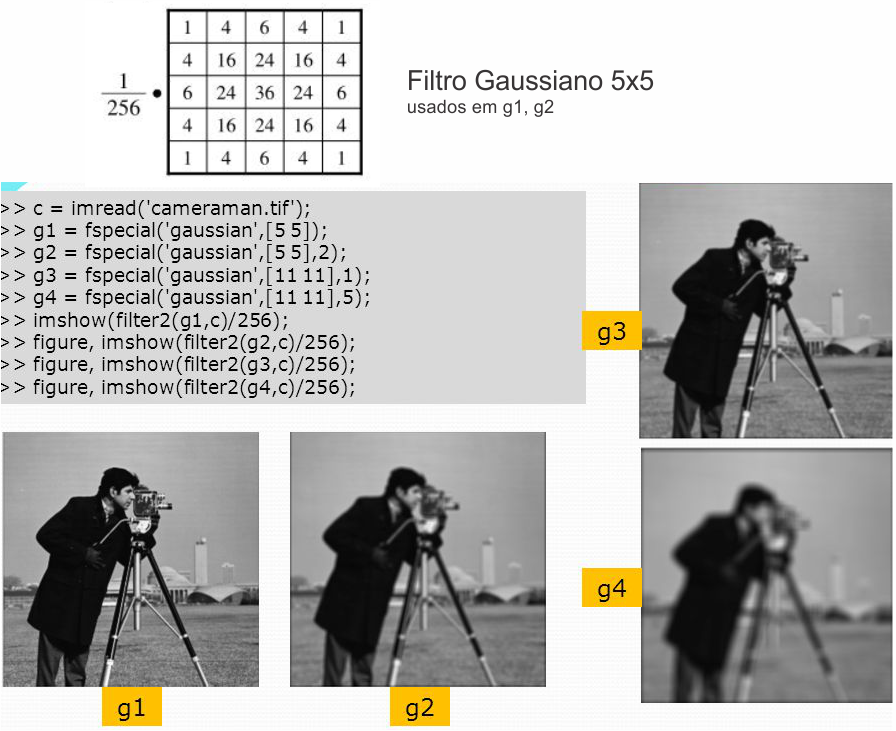
\includegraphics[scale=1.1]{questions/filter-low-pass.png}
\end{center}
\paragraph O filtro passa alta é exatamente o oposto do passa baixa, ele  faz  com que  os  detalhes  finos  da  imagem  sejam enfatizados, o tamanho da máscara (filtro) utilizada influência no resultado final, quanto menor forem as dimensões do filtro, menos detalhes serão realçados. 
\begin{center}
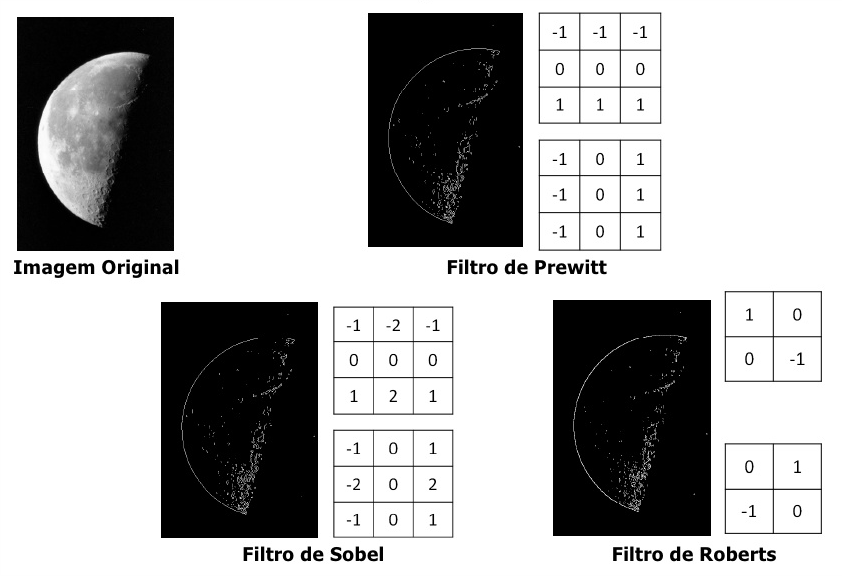
\includegraphics[scale=1.2]{questions/filter-pass-high.png}
\end{center}
%%%%%%%%%%%%%%%%%%%%%%%%%%%%%%%%%%%

% Please leave the pagebreak
\pagebreak
\paragraph{Q4:} Explain the code in file gen\_hybrid\_image\_fft.m. What each line is supposed to do? What does the function H() do?


%%%%%%%%%%%%%%%%%%%%%%%%%%%%%%%%%%%
\paragraph{A4:} O arquivo gen\_hybrid\_image\_fft.m está dividido em três etapas, obtenção da primeira imagem em baixa frequencia, obtenção da segunda imagem em alta frequencia e por fim a geração de uma terceira imagem combinando o as duas imagens ateriormente manipuladas, Os item abaixo tem por objetivo descrever as linhas de código do arquivo gen\_hybrid\_image\_fft.m.
\begin{itemize}
\item Linha 14: Declaração de um array.
\item Linha 16: Apresenta a imagem "original".
\item Linha 17: Cria um preenchimento de zeros após o termino do tamanho da imagem, em cada direção.
\item Linha 18: Converte uma imagem para double.
\item Linha 19: Convertendo para o domínio da frequência.
\item Linha 20: Desloca a imagem para o centro.
\item Linha 21: Apresenta o espectro da imagem.
\item Linha 23: Cria uma matriz de 3 dimensões.
\item Linha 24: Atribui o valor zero nas dimensões 'n' e 'm' na matriz 'h'.
\item Linha 25 até 19: Itera na matriz 'h' criando o filtro passa baixa.
\item Linha 31: Apresenta o filtro criado.
\item Linha 33: Aplica o filtro no espectro.
\item Linha 35 até 38: realiza o processo inverso, convertendo a imagem para o domínio espacial.
\item Linha 40: Atribui o resultado para o array e apresnta.
\end{itemize}

O processo é análogo para a segunda imagem, no caso teria que adicionar uma linha extra invertendo o filtro para passar somente as frequencias altas.
\begin{itemize}
    \item Linha 65: Matriz h recebe o retorno da função imcomplement dela prórpia. Esta função retorna o complemento ou negativo de uma imagem.
\end{itemize}

Por fim basta somar as duas imagens resultantes para obter o resultado final, que é a imagem hibrida.
\begin{itemize}
    \item Linha 82: Soma as duas imagens para obter a imagem hibrida.
\end{itemize}

A função H() recebe como parâmetro, as dimensões da matriz, a matriz a ser computada e o desvio padrão em pixels, o valor do desvio padrão é um dos fatores que mais impacta no resultado, em um filtro passa baixo por exemplo, quanto maior o desvio padrão, mais "borrada" fica a imagem.
%%%%%%%%%%%%%%%%%%%%%%%%%%%%%%%%%%%


% If you really need extra space, uncomment here and use extra pages after the last question.
% Please refer here in your original answer. Thanks!
%\pagebreak
%\paragraph{AX.X Continued:} Your answer continued here.



\end{document}